\section{Methods}\label{sec:methods}
\subsection{Dataset and Preprocessing}
\begin{figure}[htbp]
    %comment: this should be a different color than frequency
    \centering
    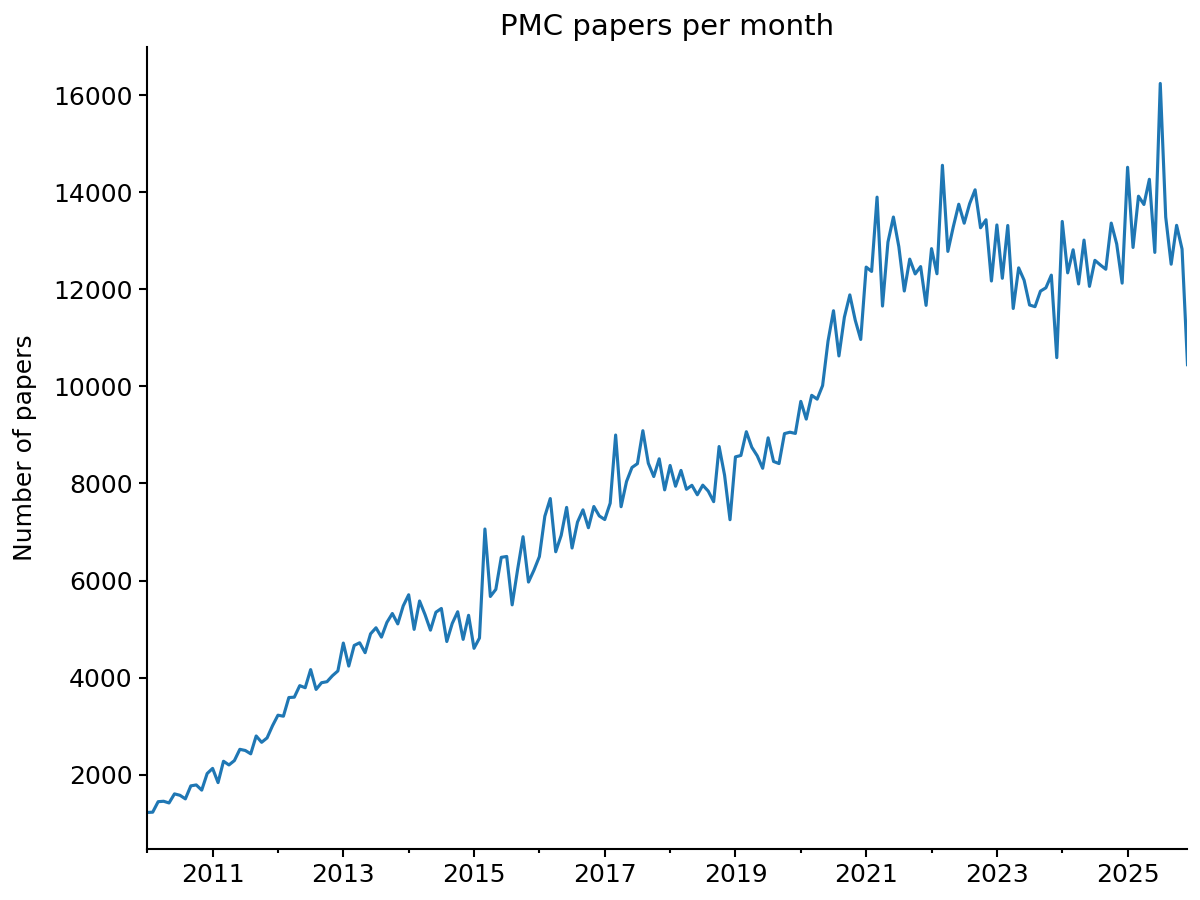
\includegraphics[width=0.7\linewidth]{../results/plots/baseline_2026-01-23/papers_per_month.png}
    \caption{}
    \label{fig:papercount}
\end{figure}
\emph{Pubmed Central}
\\
Pubmed Central (PMC) is a collection of open-access biomedical literature curated by the U.S. National Institutes of Health's National Library of Medicine \cite{pmc}. 
It provides machine-readable versions of the articles in XML format, which can be accessed individually or downloaded in bulk.
There are three open-access subsets available for bulk download with different licensing: commercial, non-commercial and other.
The latter set includes non-machine readable licenses and was therefore not used.
PMC publishes a baseline twice a year containing all papers in the collection up to shortly before the baseline's release date. 
Incremental updates are published daily in separate files.
When a new baseline is released, the previous baseline and all incremental files are replaced.
Here, we used the baseline published on January 23, 2026 containing papers dated December 31, 2025 and before.\footnote{Since work on this thesis started earlier, initial analyses used the previous baseline released June 26, 2025. These were repeated with the January 2026 baseline, so that everything reported here is based on the newer baseline}
The daily updates published after the baseline were not considered.
\\\\
\emph{XML parsing}
\\
From the XML files in the baseline, each corresponding to one paper, the following information was extracted:
\begin{itemize}
    \item Article type: specifies whether the article is a research paper, a review, a comment, etc.
    \item Date
    \item Language: only specified for a minority of papers, but is inferred later during preprocessing 
    \item Country
    \item PMC-ID: unique identifier for every paper in PMC
    \item PMID: unique identifier for PubMed, not available for every paper in PMC
    \item Journal name
    \item Title
    \item Abstract
    \item Sections
    \item Section titles
\end{itemize}
The sections and section titles are parsed from the main body of the XML file.
In general, individual sections are tagged as sec and assigned a title.
This is important for being able to compare different sections with each other, for which we need as many papers as possible with similar sections.
However, since there is no standardized format for the files, some sections are untitled or there are no section tags at all.
In particular, many files have section names for all sections except the Introduction, or don't embed the Introduction in a separate section tag. 
Therefore, if a file has more sections than section titles, and the first section is unnamed, it is assumed to be the Introduction.
Any other untitled sections are discarded.
Similarly, if there is text at the beginning of the body outside of a sec tag, it is assumed to be the introduction. 
This heuristic is not ideal, because the unnamed text contains abbreviations or keywords instead of the introduction in some cases, but since the Introduction is among the sections this study wants to focus on, it strongly increases the number of usable papers.
\\\\
\emph{Preprocessing}
\\
While some XML files specify the paper's language, this is not the case for the majority.
Since the focus here is on English text, we determine each paper's language using polyglot's detector module.
Every non-English paper is discarded.
The dates of each paper are standardized to DD-MM-YYYY format. 
Some entries only specify the month (e.g. "Feb 2025") or season of the year (e.g. "Fall 2025"), in which case the first of the month or start of the (meteorological) season are used as dates.
Papers without date are removed.
Since we want to compare LLM-use across different sections, it is important to have as many papers with comparable section structure as possible.
To achieve this, in a first step the section names were manually standardized by collecting the most frequent section names and mapping them to their standardized version.
For example, \emph{experimental results}, \emph{findings} and \emph{main results} would be mapped to \emph{results}.
If a paper has multiple sections with the same standardized title, they are concatenated.
For example, \emph{data} and \emph{experimental methods} would first both be renamed as \emph{methods} and then combined into a single \emph{methods} section.
Originally, we planned to investigate different article types and article structures, but in the end we focused only on research articles that have exactly the sections Introduction, Methods, Results, and Discussion, since papers with this article structure were the majority in the dataset.
Conversely, all papers with article types other than \emph{research-article} or with more, fewer or different sections were discarded.
Finally, all sections, including the abstract, were required to have a length of at least 250 characters.
These preprocessing steps reduce the dataset from 7,125,722 to 1,602,404 papers, 1,194,287 of which are dated 2017 or later.
\\
The use of PMC, granting us access to the whole paper, enables an extension on \cite{Kobak2025} in two regards: First, we can compare LLM-usage in the abstract to LLM-usage in the entire body of the paper, and second, we can compare different sections within the body with each other.
For this purpose, all of the analyses detailed in the following subsections were performed on the abstract, the introduction, the methods, the results and discussion of the paper, as well as the full paper, which refers to the four sections from the body without the abstract.

\subsection{Excess Frequency and LLM-use lower bound estimates}

\begin{figure}[htbp]
    \centering
    \begin{minipage}[t]{0.48\textwidth}
        \centering
        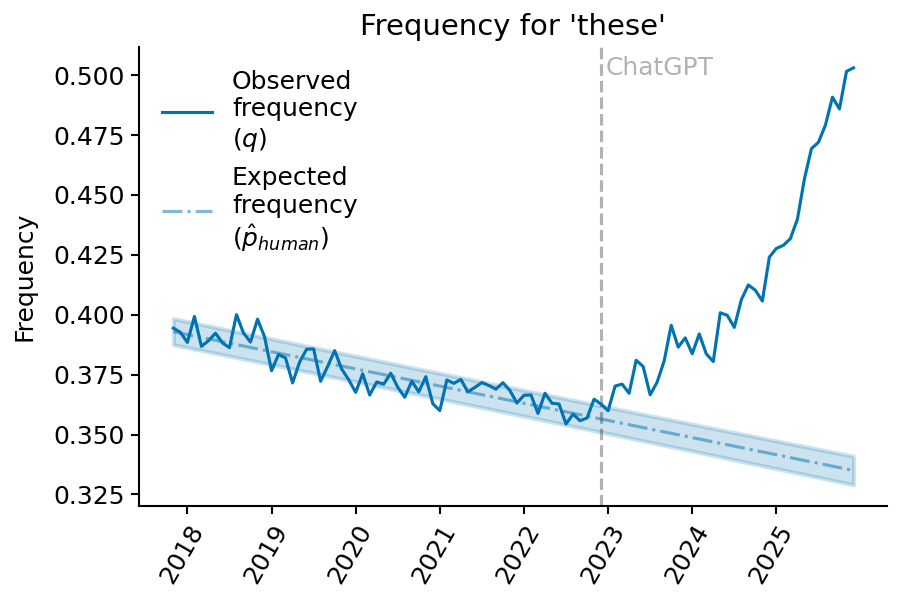
\includegraphics[width=\linewidth]{../results/plots/baseline_2026-01-23/research-article_aimrd_f/these_freqs_time.png}
    \end{minipage}
    \hfill
    \begin{minipage}[t]{0.48\textwidth}
        \centering
        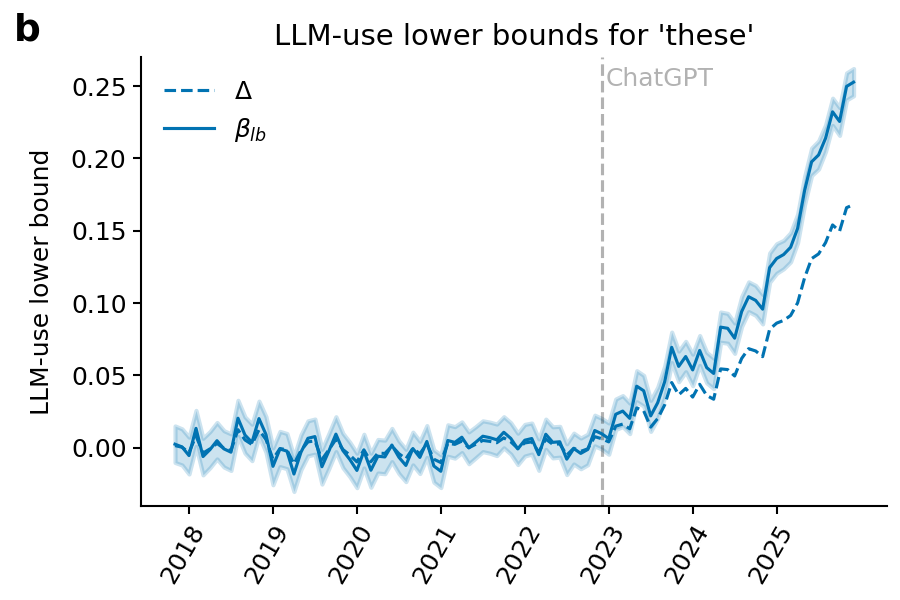
\includegraphics[width=\linewidth]{../results/plots/baseline_2026-01-23/research-article_aimrd_f/these_usage_time.png}
    \end{minipage}
    \caption{Shared caption describing both images}
    \label{fig:two_images}
\end{figure}
Excess frequency, referring to the difference between the observed and predicted frequencies for some word $w$, can be thought of as an intuitive lower bound for LLM use.
To compute it, we first determine the observed frequency of $w$.
We use sklearn's binary CountVectorizer to count the number of papers in each month or year in which $w$ occurs.
Because it is a binary count, it doesn't matter how often $w$ appears in each paper.
The vectorizer only considers words with 4 or more letters, all of which must be part of the English alphabet.
When counting word occurrence, lemmatization is an important consideration: one has to determine whether to treat different inflections of $w$ as the same or as individual words.
With lemmatization, it makes no difference if a paper contains \emph{delves}, \emph{delved} or \emph{delving}, they are all treated as an instance of \emph{delve}.
It is not immediately clear if lemmatization is helpful in this use-case.
We know from previous studies that LLMs prefer certain words.
This could imply that LLMs use all inflections of a word at a higher frequency, or that it has a strong preference for that word in a specific grammatical context (e.g. third-person singular), while using every other inflection at the same frequency in which they occur in human-written text.
As will be detailed in Section \ref{subsec:wordlist}, for the overall LLM-usage estimates, this does not matter. 
For the plots showing results for individual words, such as Figure, all word variants are included in the counts.
The frequencies are computed by dividing the monthly or yearly counts by the total number of papers in each respective time frame.
On a conceptual level, the observed frequencies $q$ are an estimate for the probability of a positive outcome in the Bernoulli trial of whether a word is present in some paper.
For dates prior to the release of ChatGPT in November 2022, marking the beginning of easily accessible LLMs, $q$ corresponds to the frequency of a word in human-written text, $p_{human}$.
After the widespread availability of Chatbots, the observed word frequency can be thought of as the product of a mixture distribution between the probability of a word to appear in human-authored and LLM-assisted text, respectively: 
\begin{equation}
    q = 
    \begin{cases}
        p_{human} & \text{for papers before 11-2022}\\
        (1-\beta) \cdot p_{human} + \beta \cdot p_{LLM} & \text{for papers after 11-2022}\\
    \end{cases}
\end{equation}
The mixture component $\beta$ in the lower case indicates the proportion of papers that were written with the help of LLMs.
We can transform this equation to obtain an expression for $\beta$:

\begin{equation}\label{eq:beta}
\begin{split}
    q &= (1-\beta) \cdot p_{human} + \beta \cdot p_{LLM}\\
    \beta \cdot (p_{LLM}-p_{human}) &= q -  p_{human}\\
    \beta &= \frac{q -  p_{human}}{p_{LLM}-p_{human}}
\end{split}
\end{equation}
\\
While $p_{human}$ can be estimated by the observed $q$ in the time span before November 2022, there is no direct way to do so after the release of ChatGPT.
However, if we assume that human usage of words follows linear trends and is independent of LLM-use, we can use the values before 2022 to model $\hph$ using linear regression.
Since we are interested in both the monthly and yearly trends, we fit the regression either on the five yearly frequency values from 2018 to (including) 2022, or on the 60 monthly frequencies from November 2017 to October 2022.
For the yearly data we include 2022 in the train set because, considering the time it takes to write a paper, and the time it took the new technology to gain traction, it is unlikely that many papers published in December 2022 were written with the help of LLMs.
Replacing the unknown $p_{human}$ with the estimate $\hph$ in equation \ref{eq:beta}, one issue remains: there is no direct way to estimate $p_{LLM}$ from the observed frequencies.
The others solve this problem by using ground-truth LLM-generated text to determine $p_{LLM}$.
Here, we choose a different approach by determining a lower bound for $\beta$ that doesn't rely on $p_{LLM}$:
\begin{equation}\label{eq:delta}
    \begin{split}
        \beta &= \frac{q -  \hph}{p_{LLM}-\hph}\\
        \beta &\ge q - \hph =\Delta
    \end{split}
\end{equation}
This is the excess frequency measure introduced by \cite{Kobak2025} and denoted $\Delta$.
Intuitively, if a word appears in $70\%$ of papers in 2025, but we predict humans to use this word in only $60\%$ of instances, the $10\%$ gap must be accounted for as having been written by LLMs. 
Note that this metric will lead to a strong under-estimation of the actual LLM usage, because a human-use frequency of $60\%$ will only translate to $60\%$ of observed use, if all texts in the sample are in fact written by humans ($\beta=0$).
In reality, some papers were written with the help of LLMs, such that the fraction of word-occurrence that can be explained by human usage is not $60\%$ of all papers, but $60\%$ of the papers with human authorship.
A stronger lower bound, denoted $\hbet$ is also possible:
\begin{equation}\label{eq:beta_hat}
    \begin{split}
        \beta &= \frac{q -  \hph}{p_{LLM}-\hph}\\
        \beta &\ge \frac{q -  \hph}{1-\hph} = \hbet
    \end{split}
\end{equation}
In dividing by $1-\hph$, this lower bound readjusts the estimate by focusing only on the fraction of papers for which no human use of the word is to be expected.
In the above example with $p_{human}=60\%$ and excess frequency of $\Delta=10\%$, $1-\hph=40\%$ of papers wouldn't contain the word if there were no LLM-authored texts, but only $1-q=30\%$ actually don't, so the remaining $\frac{10\%}{40\%}=25\%$ must be LLM-authored.  

\begin{figure}[htbp]
    \centering
    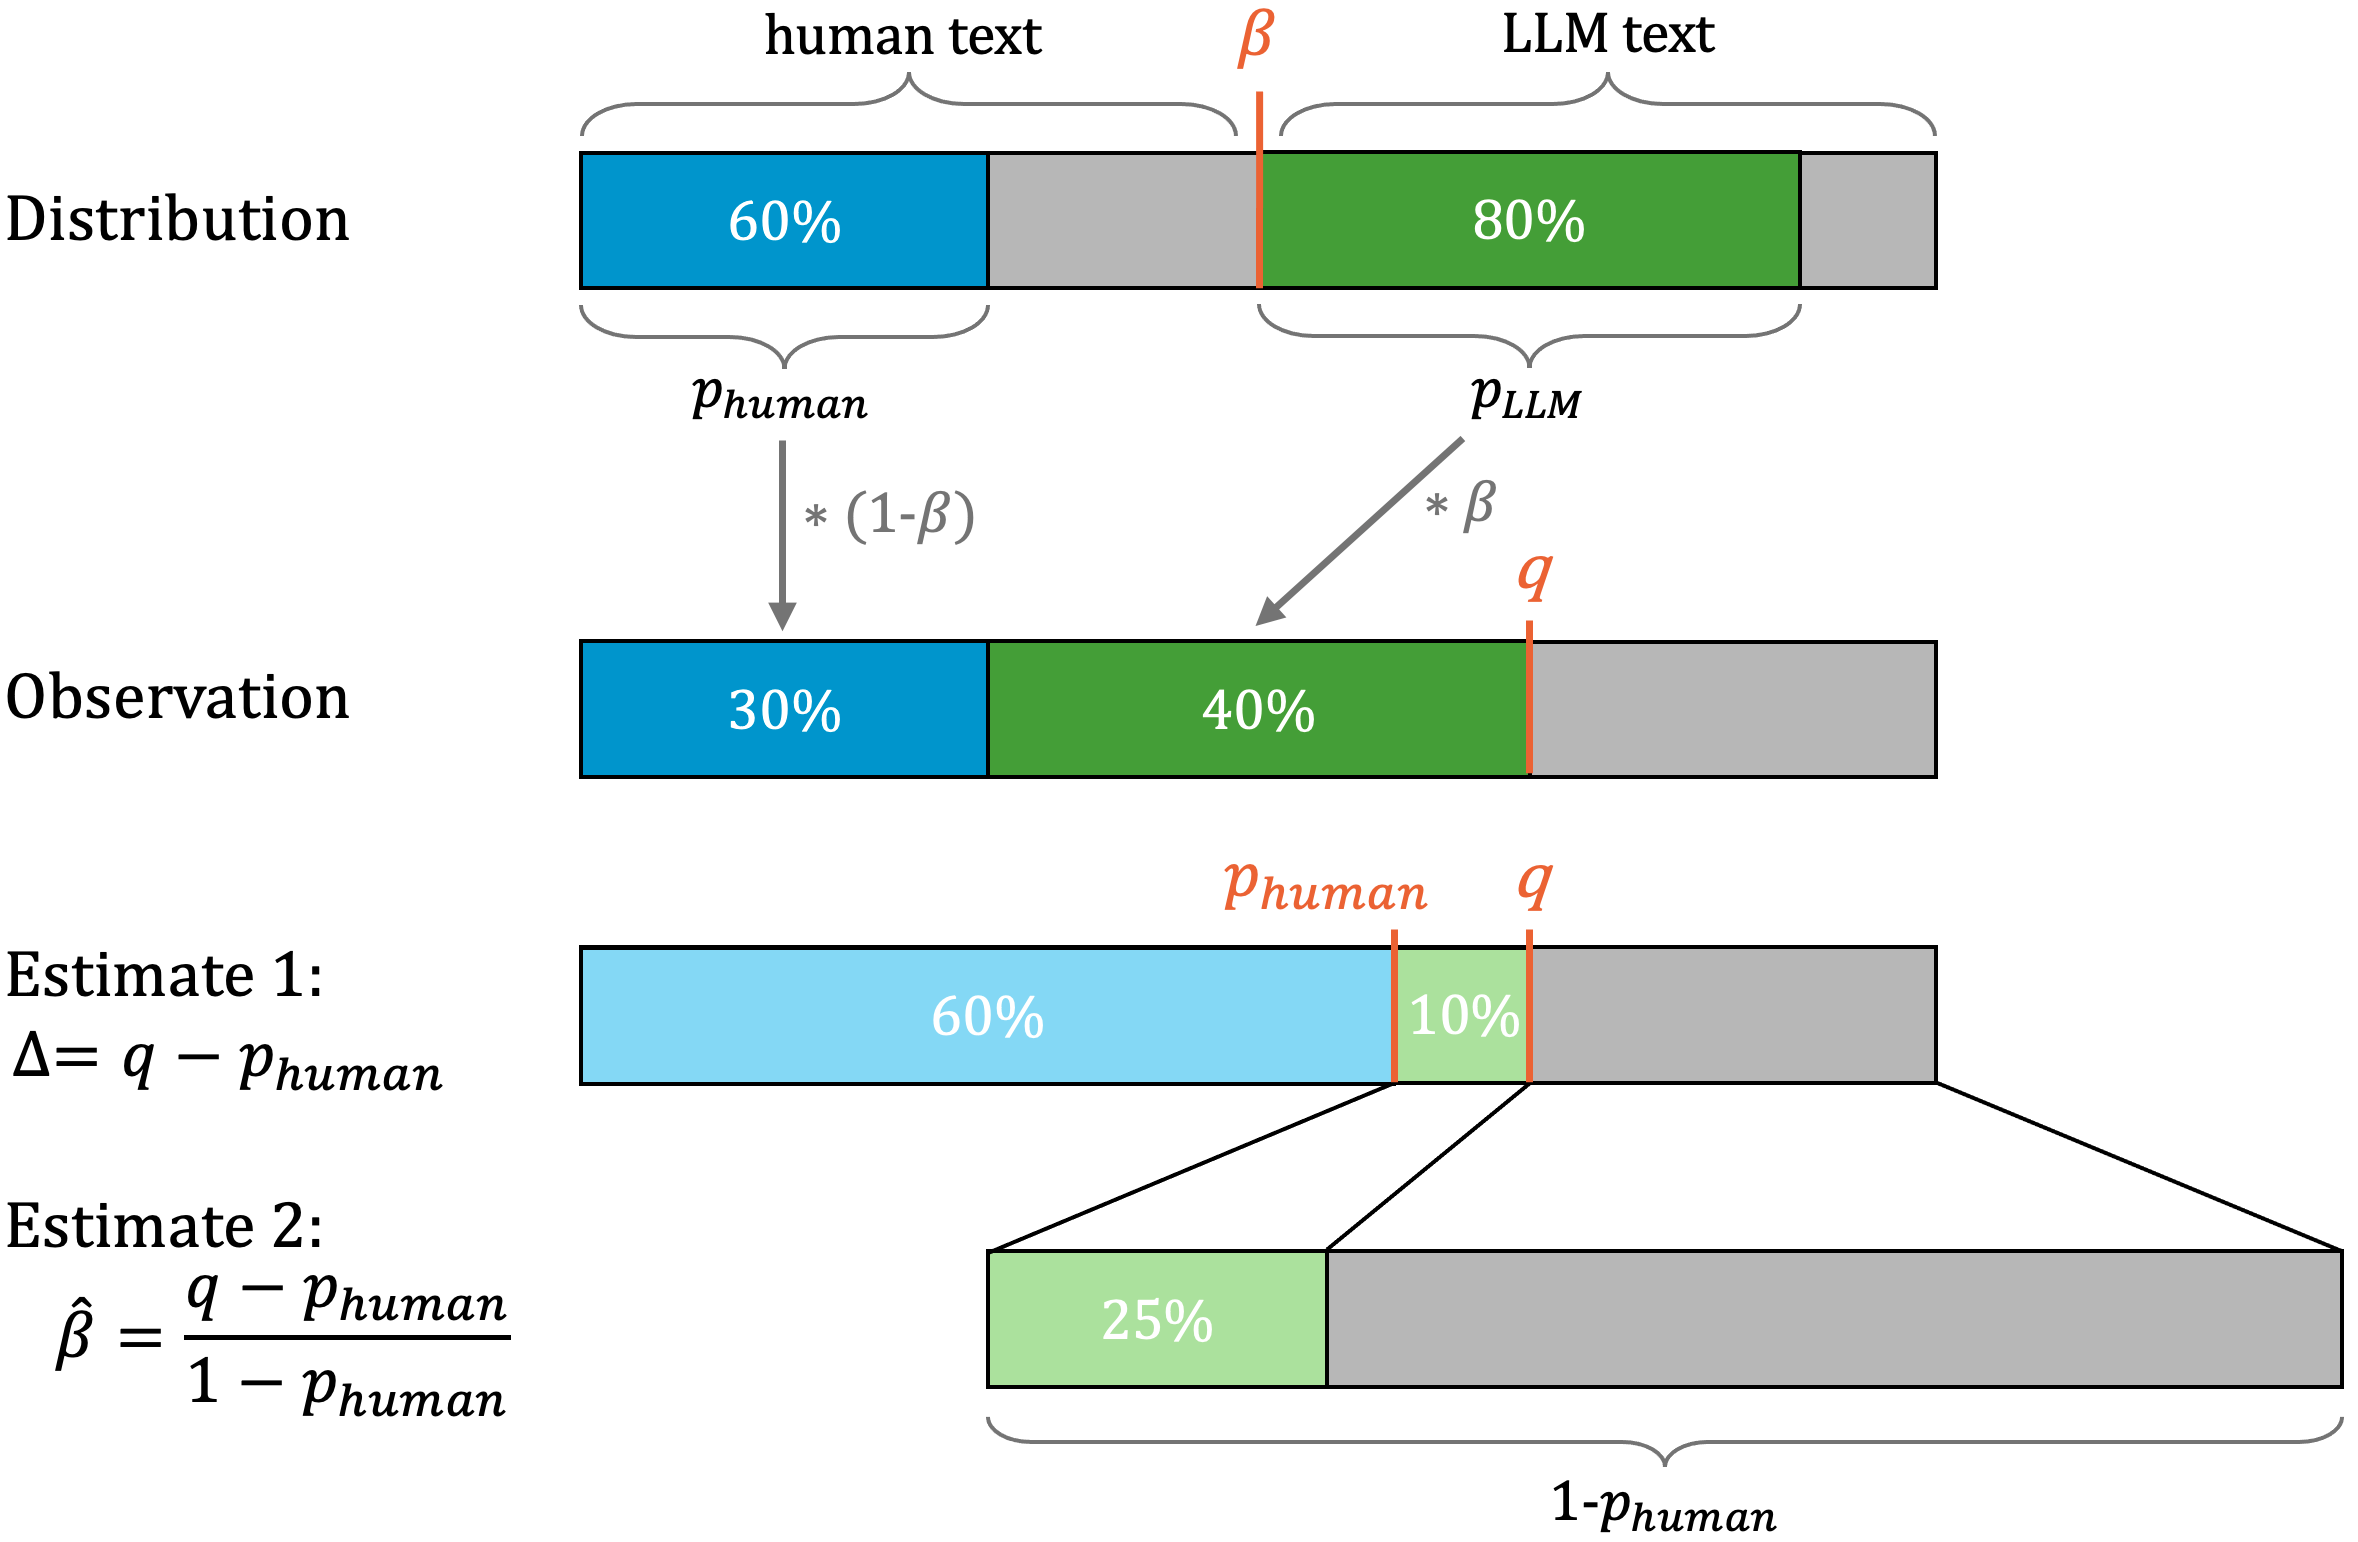
\includegraphics[width=0.7\linewidth]{../results/plots/misc/intuition_estimate_v2.png}
    \caption{}
    \label{fig:intution_estimates}
\end{figure}



\subsection{Grouped word frequencies}\label{subsec:wordlist}
\begin{figure}[htbp]
    \centering

    \begin{minipage}[t]{0.48\textwidth}
        \centering
        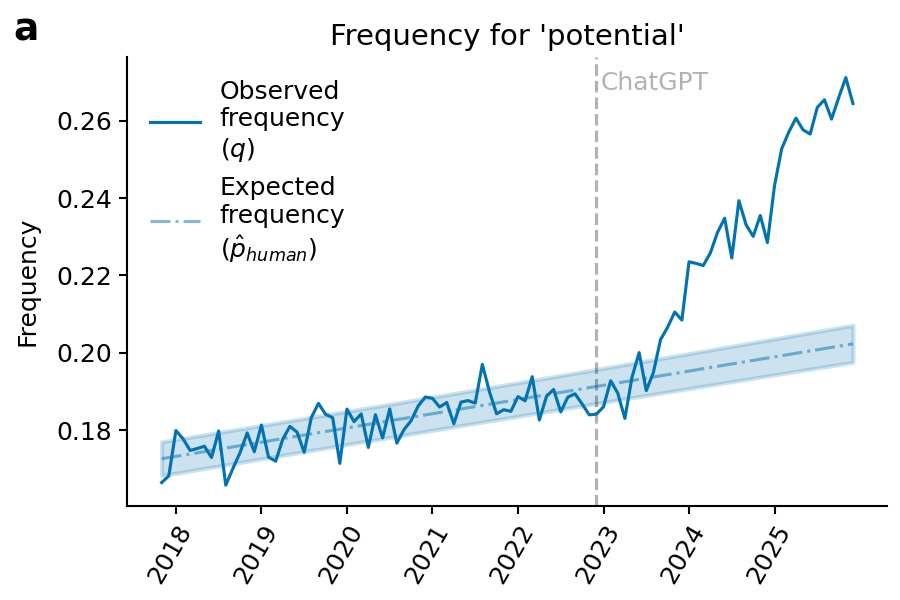
\includegraphics[width=\linewidth]{../results/plots/baseline_2026-01-23/research-article_aimrd_f/potential_freqs_time.png}
    \end{minipage}
    \hfill
    \begin{minipage}[t]{0.48\textwidth}
        \centering
        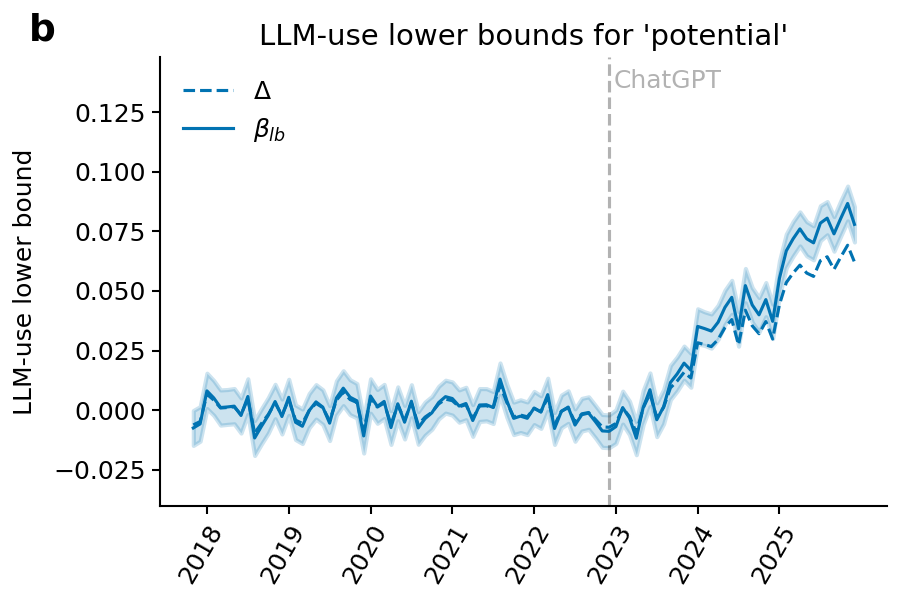
\includegraphics[width=\linewidth]{../results/plots/baseline_2026-01-23/research-article_aimrd_f/potential_usage_time.png}
    \end{minipage}

    \medskip

    \begin{minipage}[t]{0.48\textwidth}
        \centering
        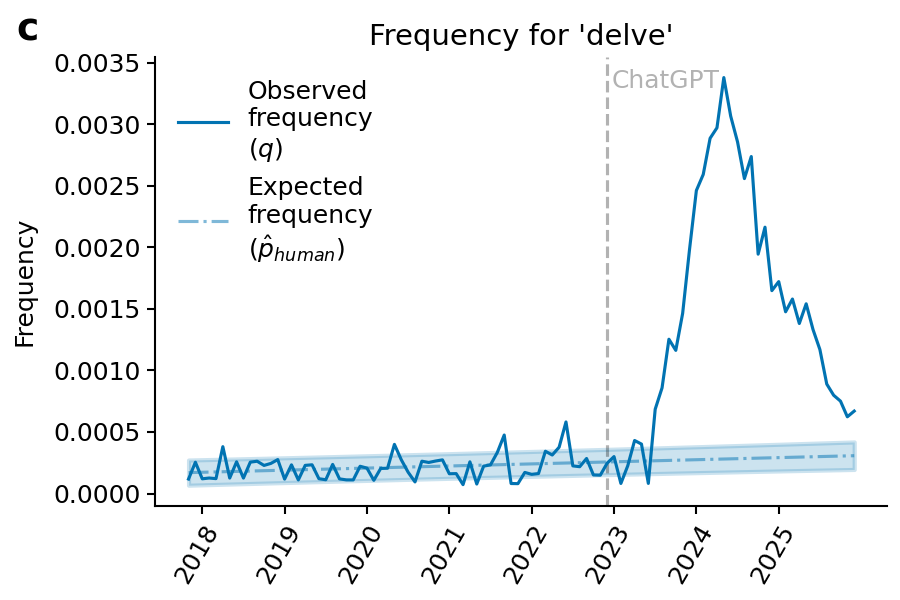
\includegraphics[width=\linewidth]{../results/plots/baseline_2026-01-23/research-article_aimrd_f/delve_freqs_time.png}
    \end{minipage}
    \hfill
    \begin{minipage}[t]{0.48\textwidth}
        \centering
        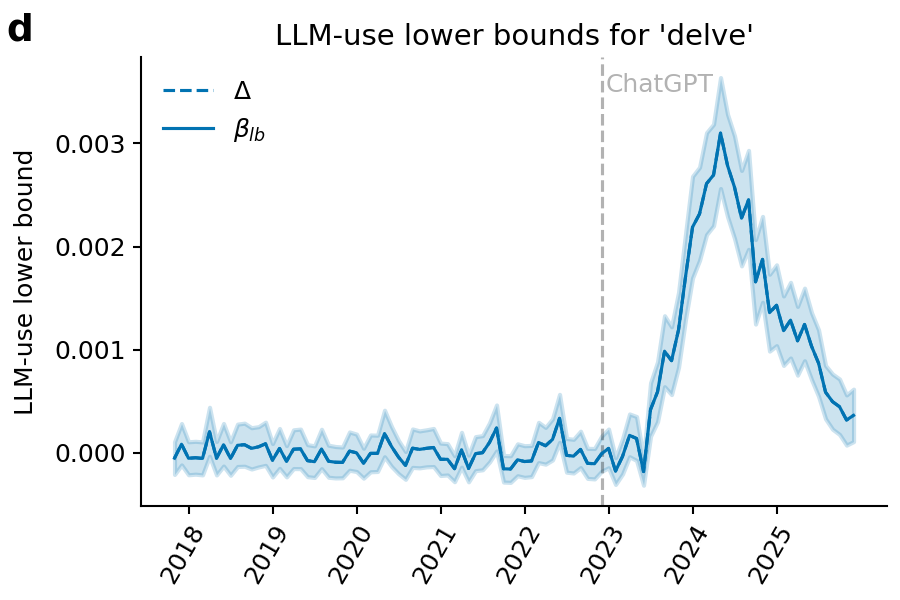
\includegraphics[width=\linewidth]{../results/plots/baseline_2026-01-23/research-article_aimrd_f/delve_usage_time.png}
    \end{minipage}

    \caption{Fix title for delve estimates!}
    \label{fig:four_images}
\end{figure}

While single words are useful to illustrate the concept of excess frequency, they are suboptimal as a basis for an accurate estimate of overall LLM-use.
The reason for this is obvious: while LLMs might use a word such as ``potentially'' at a higher frequency than humans would, ``potentially'' doesn't fit in every context so there will potentially be a lot of LLM texts not containing it.
Also, the observed frequencies of some words might be unreliable.
The word ``delve'', used as the titular example of excess vocabulary in \cite{Kobak2025}, has experienced a sharp decline in popularity starting around mid-2024, when it was widely reported as an example of ``LLM-speak''.
Many authors have thus moved to using word lists as markers. 
The method of computing the frequencies doesn't change, but instead of counting in how many papers a single word appears, we count in how many papers at least one of the words in the list appears.
The most systematic way to create a list of words indicative of LLM-use is to use a data-driven approach, which doesn't require a manually selected list.
\\\\
\emph{Excess words for 2024 PubMed}
\\
\cite{Kobak2025} determine the excess words for 2024 by computing the frequency gap and the frequency ratio for each word in their dataset.
The frequency gap is the same metric as $\Delta$ in Equation \ref{eq:delta}, although they only use the yearly frequencies of 2021 and 2022 to predict $\hph$.
The frequency ratio is computed as $\frac{q}{\hph}$.
An excess word is defined as any word with frequency gap or frequency ratio above a certain threshold.
The thresholds were chosen in such a way that the majority of words in texts from the years 2012 - 2023 were excluded
(The gaps for previous years were also computed by comparing observed values to $\hph$ computed based on two and three years prior).
Using both metrics as inclusion criteria serves to increase the number of excess words.
For instance, a word whose usage increases from 0.0001 to 0.001 will have a relatively small gap but a large ratio, while a word whose prior frequency of 0.3 rises to 0.4 has a large gap with a relatively small ratio. 
Both changes mark a notable difference in usage and should therefore be candidates for marker words.
All words above the threshold were then manually annotated as \emph{style words} or \emph{content words}.
\emph{Content words} are all words related to the research topic of a certain paper. 
Their excess use can be attributed to new inventions or research trends.
Examples include ``RNN'' in 2018, ``Covid'' in 2020, and ``ChatGPT'' in 2024.
\emph{Style words}, on the other hand, are not related to research topics and could be found in any discipline: ``these'', ``potentially'', ``delve'', etc.
Excess words of 2024 were defined as all style words with frequency gap or ratio gap above the respective thresholds.
This resulted in a list of 379 words, which can be found in the Appendix \ref{ap:wordlist}.
\\\\
\emph{Optimal word lists}
\\
The excess word list can be used to create the optimal list of marker words to detect LLM-use.
It might be counter-intuitive to not just use the whole list: if any of the words can act as a marker for LLM-use, then using as many words as possible should yield the most accurate result.
However, one has to keep in mind that all excess words also appear in human-written text.
If there are too many words in the list, their cumulative frequency will be close to 1 even for $p_{human}$.
For \cite{Kobak2025}, who use the frequency gap $\Delta$ as their LLM-use estimate, this is suboptimal because the closer $\hph$ is to 1, the smaller the potential gap.
When using $\hbet$ as the metric, the best estimate would be achieved by getting $p_{LLM}$ as close to 1 as possible, which would in turn move $\hbet$ closer to the true value $\beta$.
While $p_{LLM}$ isn't observable, it can be manipulated by increasing the number of words in the excess list.
However, this also includes the caveat that $\hph$ must remain smaller than 1, otherwise, Equation \ref{eq:beta_hat} yields division by zero.
This means that for both estimates, $\Delta$ and $\hbet$, a subset of the 2024 excess words needs to be determined.
Because brute-forcing the decision on an optimal list by trying all possible combinations is not feasible, \cite{Kobak2025} sorted the excess words by their individual frequencies in 2024 (lowest to highest), and then used different cutoff values to create subsets of all words whose individual frequencies were below the cutoff. 
Each resulting list was used to compute the LLM-use estimate $\Delta$ and the highest $\Delta$ was used as the final estimate.
\\\\
\emph{Adaptation to PMC data}
%comment: include graph of excess words for one section? also include the paper composition?
Initially, we planned to repeat the procedure of finding excess words for the PMC dataset.
This turned out to be non-feasible, because the length of the full papers, as opposed to only abstracts, lead to a huge number of excess words, which would all have to be manually annotated to filter them for style words.
Instead, we used the previous study's 2024 excess word list.
This is permissible because, first, PMC is a subset of the PubMed data used in \cite{Kobak2025}, so the domain is similar, and second, the point of using style words is to have marker words that are domain-independent.
(Although it is likely that when searching for excess words in a different domain, such as news articles, the resulting list would be somewhat different).
The 2024 excess word list is not lemmatized, so that ``delving'' and ``delves'' are treated as different words.
Since we are not interested in the excess words on a semantic level and use them only as indicator of LLM use, it does not matter if two words on the list are variations of the same verb, or if a third variation of the verb is not included.
To get the optimal list for each section, we sort the 2024 excess words by their individual frequency in 2024.
This leads to a somewhat different order for each section.
Like in the previous work, we then use different cutoff values to create subsets of excess words, which serve as a basis for computing the LLM-use estimate $\hbet$.
We started with x cutoffs spaced evenly on a log-scale between 0 and 1 and later added intermediate values in the high-interest region around the maximum, resulting in y cutoffs.
Initially, we used the same approach as above to select the maximum $\hbet$-value as the estimate.
However, in some cases, the maximum was at one of the highest cutoff value, leading to nearly the full excess word list being used for the estimate.
This results in values for $q$ and $\hph$ that are extremely close to 1, sometimes with $\hph$ being larger than $q$, which contradicts the assumption $p_{human} < p_{LLM}$.
As a consequence, both numerator and denominator of the fraction $\frac{q - \hph}{1-\hph}$ are very close to 0, which can lead to unstable behavior.
To prevent this, any cutoff that leads to estimates of $\hph \ge 0.999$ was excluded as candidate for creating optimal excess word lists.
%comment: check this number and include plot that shows oscillation of estimates that go too close to 1
\\
The optimization was performed on yearly frequency data separately.
This means that the optimal cutoff for 2024 could be different to that of 2025.
For the main analysis, the optimal cutoff values for 2025 were used for all time points to simplify procedure and have more easily comparable results.
Notably, the main analysis was performed on monthly data with the word lists optimized for the year 2025, instead of optimizing each month individually, for simplicity.
A possible approach with optimizing on monthly intervals of the data would be to take the majority optimum as the list for all estimates.
The end result would be the same: Some time intervals would be estimated with the optimal word list, while others wouldn't.
\\
To better judge the reliability of the estimates, we computed the standard error and performed sanity checks using simulated frequency data.

\subsection{Method validation}
\emph{Standard error for LLM-use estimates}
Since the LLM-use estimate $\hbet=\frac{q -  \hph}{1-\hph}$ depends on $\hph$ and $q$, we first need to determine their respective errors, before propagating them to obtain the error for $\hbet$.
We conceptualize $q$ as the maximum likelihood estimate (MLE) for the binomial probability of a word from the excess word list to appear in a paper.
As such, the MLE's variance is $SE_q^2=\frac{q(1-q)}{n}$, with $n$ as the number of papers in the current month or year.
$\hph$ is the regression estimate of a binomial probability. 
Since $\hph$ is not an empirical estimate, the binomal MLE variance doesn't apply and we focus on the regression variance.
Technically, the data points that the regression was trained on are empirical estimates (since training was done on $q$ values in the time span before the release of ChatGPT).
To factor in this binomial maximum likelihood uncertainty, it should be included in the regression formula.
However, because the MLE variance is very small due to the large number of papers each month, this was omitted for simplicity.
The regression variance for design matrix $X$ (including only points on which the regression is fit, corresponding to the time before the release of ChatGPT), predictor matrix $x$ (including all points that are to be predicted, including pre- and post-ChatGPT frequencies) and response vector $y$ is computed with the following formula:
\begin{equation}
    SE_{\hph}^2= \hat{\sigma}^2 x(X^TX)^{-1}x^T + \hat{\sigma^2}
\end{equation}
with $\hat{b}=(X^TX)^{-1}X^Ty$ as the estimated regression coefficients\footnote{As per common convention, the estimated regression coefficients are normally denoted $\hbet$, which was changed to $\hat{b}$ to avoid confusion with the LLM-use estimate $\hbet$}
and $\hat{\sigma}^2=\frac{\|y-X\hat{b}\|^2}{n-2}$ the unbiased estimate of the noise variance, where $n$ refers to the number of papers, of which the number of predictors, 2, is subtracted.
$\hat{\sigma}^2x(X^TX)^{-1}x^T $ is the covariance matrix of the regression coefficients, specifying the uncertainty of the mean prediction. 
To this, an additional $\hat{\sigma}$-term is added to estimate how far the predicted values would have deviated from this mean.
\\
The variance of $\hbet$, as a nonlinear function of $q$ and $\hph$, is not trivial to determine.
We can apply the Delta method, which uses Taylor series approximation, to do so.
We assume $q$ and $\hph$ to be the means of random variables $Q$ and $P$, respectively.
First, we approximate $\hbet((Q,P))$ around the mean $\mu=(q, \hph)$ with a first-order Taylor expansion:
\begin{equation}
    \hbet((Q,P)) \approx \hbet(\mu) + \nabla\hbet(\mu)^T((Q,P)-\mu)
\end{equation}
with gradient $\nabla$ as
\begin{equation}
    \nabla \hbet(\mu)= \left[ \frac{\partial\hbet}{\partial q}, \frac{\partial\hbet}{\partial \hph}\right]^T = \left[ \frac{1}{1-\hph}, \frac{q-1}{(1-\hph)^2}\right]^T 
\end{equation}
We can use this to compute the variance of $\hbet$:
\begin{equation}
    \begin{split}
        Var(\hbet) &= Var(\hbet(\mu) + \nabla\hbet(\mu)^T((Q,P)-\mu)\\
        &= Var(\hbet(\mu) + \nabla\hbet(\mu)^T(Q,P)-\nabla\hbet(\mu)^T\mu)\\
        &= Var(\hbet(\mu)^T(Q,P))\\
        &= \nabla\hbet(\mu)^T\Sigma\nabla\hbet(\mu)
    \end{split}
\end{equation}
We assume independence of the two random variables $Q$ and $P$, so that the covariance matrix $\Sigma$ only has the diagonal entries of the estimate variances $SE_q^2$ and $SE_{\hph}^2$ derived above. 
We excluded all estimates with a standard error of $SE_{\hbet}\ge 0.025$.
%comment: the error bars don't work if p is 1 (or veryvery close to 1), because in that case, binomial error is 0
\\\\
\emph{Sanity check simulation}
\\
\begin{figure}[htbp]
    \centering
    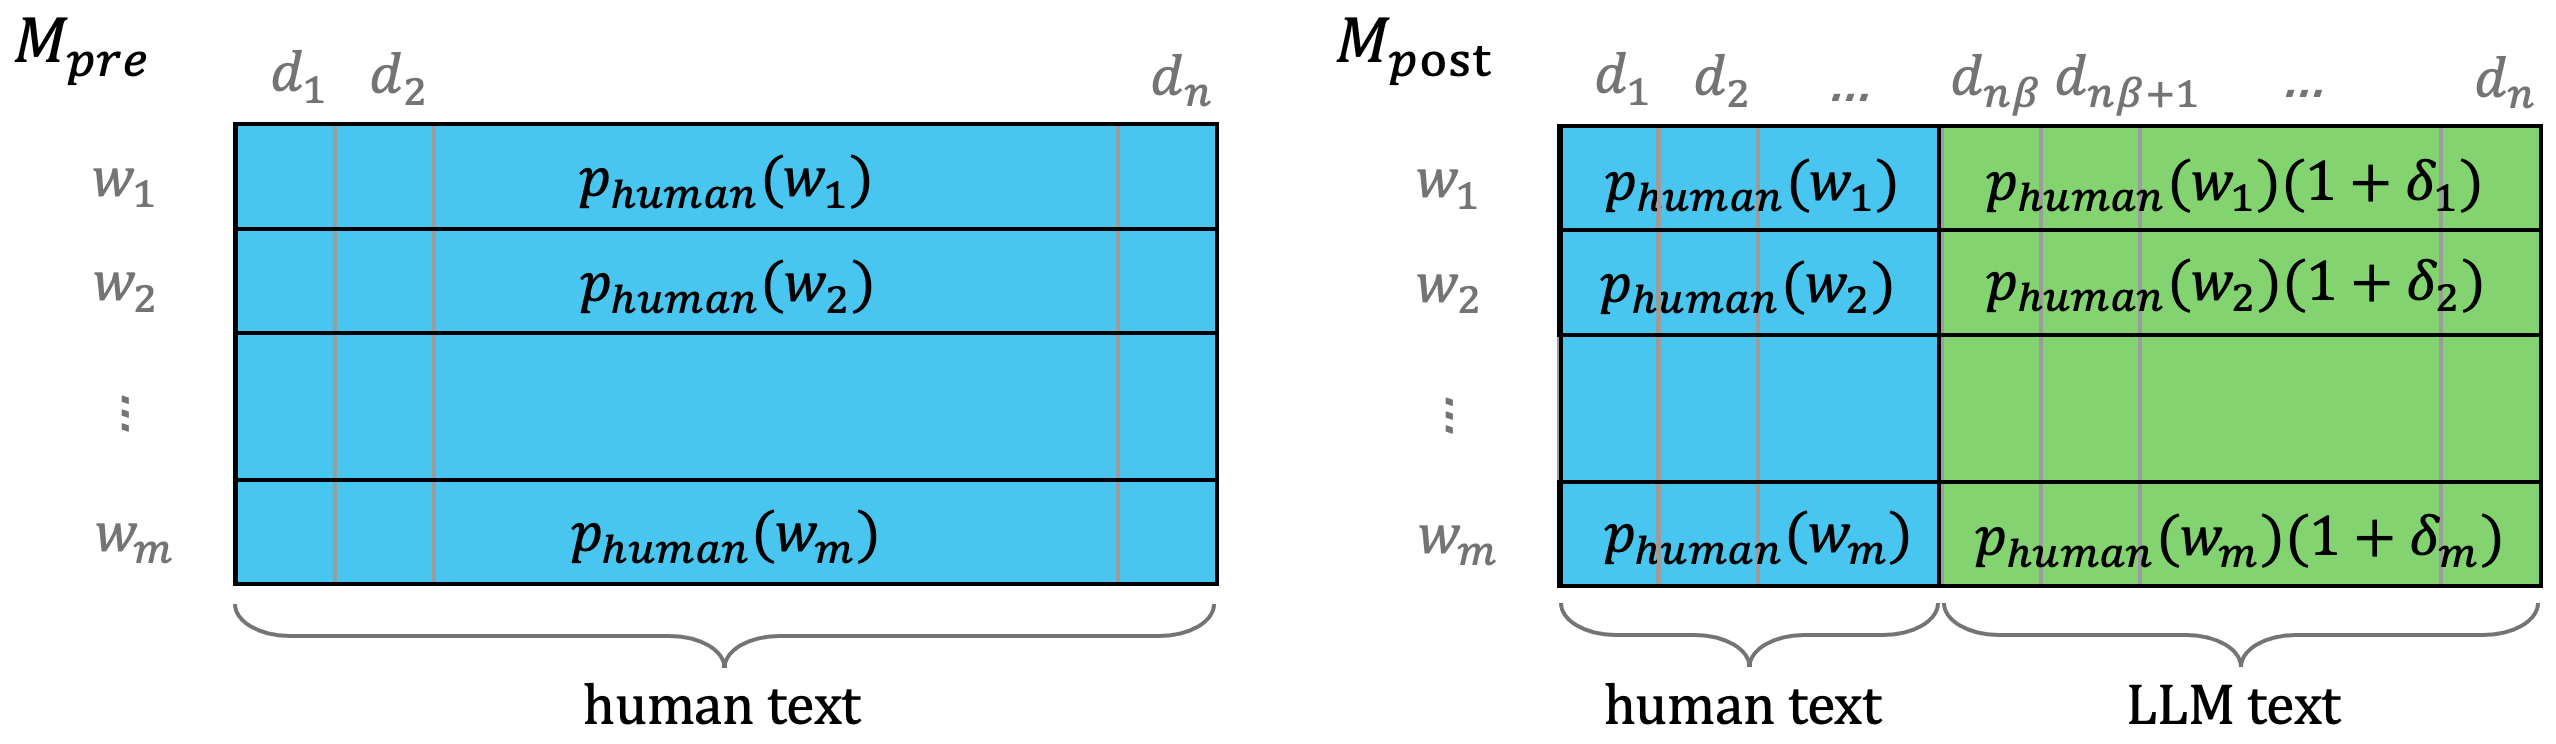
\includegraphics[width=0.9\linewidth]{../results/plots/misc/intuition_simulation_v2.png}
    \caption{Illustration of the sampling procedure for the creation of an artificial dataset to test the LLM use estimate $\hbet$ for varying levels of $\beta$}
    \label{fig:intution_simulation}
\end{figure}
To better gauge how well the procedure of finding the optimal excess word list to get the best possible lower bound works, we performed the same analysis on simulated data with known $\pl$ and $\ph$ and varying $\beta$.
We simulated data for 100,000 texts, approximating the number of papers per year in our sample.
In our simulation, there were 500 words, all of which were treated as excess words.
We created two matrices, $M_{pre}$ and $M_{post}$, each with dimensions (\emph{number of texts, number of words}), corresponding to data before and after the release of ChatGPT, respectively.
For $M_{pre}$, each word $w$ was randomly assigned a probability $\ph(w)$. 
The probabilities were sampled from a gamma distribution with shape parameter $2$ and scale parameter $0.02$.
Then, 100,000 binomial samples were drawn with $\ph(w)$ as probability of success for each word.
For $M_{post}$, a fraction of $\beta$ texts were selected as being LLM-generated.
As one of the assumptions posits that $\ph\le\pl$, the probabilities for words to occur in LLM-assisted text were sampled as $\pl(w)=\ph(w)(1+\delta)$, with $\delta \sim U(0.5,5)$.
In cases where $\ph(w)(1+\delta)>1$, $\delta$ was newly sampled until the resulting $\pl(w)$ was in the range $[0,1]$.
In the sampling process $100,000\cdot \beta$ binomial samples were drawn with probability $\pl(w)$, and $100,000\cdot (1-\beta)$ were drawn with probability $\ph(w)$.
\\
For the following analyses, the word frequencies in $M_{pre}$ was treated as analogous to $\hph$, and those in $M_{post}$ as the observed frequencies $q$.
The words in $M_{pre}$ were ordered by frequency, and excess lists were formed of words with frequencies lower than those of several different cutoffs. 
For each excess list corresponding to one of the cutoffs, the LLM-use estimates $\Delta$ and $\hbet$ were computed.
The only difference w.r.t. the procedure on the real data was during variance computation: $M_{pre}$, as opposed to $\hph$, is not the result of a regression, but, similar to $q$ the result of a binomial sampling procedure. 
Thus, the variance for frequencies based on $M_{pre}$ was computed as the variance of a binomial estimator, $Var(M_{pre}) = \frac{p(1-p)}{n}$ with $p$ the observed frequency and $n=(1-\beta)\cdot n_{texts}$.
As with the real data, we exclude cutoffs yielding frequencies $\ge0.999$ for $M_{pre}$, as well as estimates with error bars $\ge0.025$.


\subsection{Section length}
One of the goals of this project was to compare the estimated LLM-use of different sections of the paper with each other.
This might seem like an unfair comparison: When using word occurrence as LLM-marker, longer texts are at an advantage - there is simply more space for words to appear in.
[Figure here shows the different section lengths]
For example, if an LLM produced some word once every 500 words on average, it would appear in the majority of 1000-word sections, but only in about half of 250-word sections, despite all of them being written by an LLM.
Since the word counts are binary, there is no correction for section length in the estimate.
This is a further argument for using section specific word lists instead of single words.
The longer the word list, and the higher their aggregated frequency, the less likely it is for an LLM-generated text, however short, to not contain at least one of them.
However, when authors use LLMs, it is also likely that they focus their usage on specific paragraphs that they, e.g., wish to rephrase.
A longer section contains more paragraphs that might warrant re-working.
One way to address this issue is to slightly shift the question from \emph{How high is LLM-use in this section?} to \emph{How high is LLM-use in a random paragraph of this section?}
% By focusing on paragraphs instead of full sections, the section length can be controlled for. 
This was implemented by cropping each section sample to a length of 255 words, which corresponds to the median length of the abstracts.
The cropped part was placed randomly within the section by sampling a starting position ranging between the first and 255th-last words in the text.
Note that the LLM-use estimate based on the cropped sections can't be used to determine the full fraction of papers that were written with some LLM participation.
Since we are interested in identifying not only those papers that are wholly written by an LLM, using only one paragraph per section will underestimate the number of papers written with the help of LLMs, because this paragraph might not include the parts of the paper where LLMs were used. 
However, by comparing the results from the full and cropped sections, we can check whether LLMs are used universally across the entire paper or whether their use is concentrated on some paragraphs.



\subsection{Subgroup analysis}
%comment: add plot with number of paper per country (barplot for ind country counts, say 2017 to 2025, pie chart with entries "english-speaking", "non-english speaking", "unknown country")
Another point of interest is how LLM-use differs across subsets of the data.
It is, for instance, plausible to assume that majority English-speaking countries will show different usage patterns than countries where English is learned as a second language.
Likewise, there might be differences between academic disciplines, with some being quicker to adopt a new technology.
Previous studies typically reported higher usage estimates for research areas related to computer science.
To compare these categories, we repeated the experiments on different subsets of papers.
\\\\
\emph{Countries}
\\
The most salient criterion to compare countries with each other when it comes to LLM-use is their majority native language.
Since English is the de facto lingua franca of academia, one of the key capabilities of LLMs is their ability to translate or proofread text from authors uncertain of their English proficiency.
As this use-case is irrelevant for native English speakers, it stands to reason that LLM-usage would be smaller for English-speaking countries.
\\
To categorize countries into English and non-English speaking, we used the \emph{Three circles of English model}\cite{kachru1985standards}, which sorts the United States, the United Kingdom and Ireland, Australia and New Zealand, South Africa, and the majority of Canada into the ``inner circle'', where English is the native language of the majority of inhabitants and primarily used in their day-to-day lives.
All other countries were classified as non-English speaking. 
Additionally to comparing English to non-English speaking countries, we also analyzed the LLM-use of individual countries.
We selected the 18 countries with highest paper counts in the years 2017 to 2025.
The full list of countries and their respective paper counts can be found in the Appendix.
\\
We originally planned to use the excess word lists that are optimal for each section with regards to the full dataset. 
However, this lead to observations of $q=1.0$ for several years and countries (pre- and post-release of ChatGPT).
Due to time constraints, it was unfeasible to search for the optimal list for every country and section.
As a heuristic to approximate the search process, the list corresponding to the next-lower cutoff was selected.
For example, for the abstract, the optimal cutoff was $0.1$, so we selected the list corresponding to a cutoff value of $0.07$, which was the value directly preceding $0.1$.
By lowering the cutoff, we reduce the number of words in the excess word list and can thus regulate the observed frequencies.
This ``suboptimal'' cutoff also lead to problematic observations, because in many cases, $q$ was within the regression error of $\hph$, which is not ideal for any metric depending on the difference between the two.
To adjust, we moved the cutoff value one position further down, e.g. by going from $0.1$ to $0.05$ instead of $0.7$ for the abstract.
\\\\
\emph{Research disciplines}
\\
%comment same plot as for countries, maybe put in appendix? or do table instead of plot?
Papers were sorted into different research areas based on the titles of journals in which they were published in a procedure based on \cite{gonzalez2024landscape}.
The research areas are subfields of the biomedical domain, for example radiology or nursing, that were specified in \cite{gonzalez2024landscape}.
The full list of categories can be found in the Appendix.
Journals were sorted into a category via keyword search with the category titles, and were assinged no label in case of no match.
This is a relatively crude but simple approach that ignores many potential matches, e.g., the (hypothetical) \emph{Journal of Neurology} would be assigned the label ``neurology'', while the \emph{Neurological Journal} would not. 
The number of matches could be improved by using fizzy matching or manually annotating 
In assigning labels, the keyword appearing latest in the title was given precedence. 
For example, the \emph{Journal of Cancer Biochemistry} would be sorted into the ``biochemistry'' category, while \emph{The Biochemistry of Cancer} would be assigned the label ``cancer''.
This procedure resulted in 23\% of papers being labeled.
Only labels with more than 5000 papers were selected for further analysis.
Using the optimal excess word lists to compute frequencies lead to similar problems as detailed above, which is why we also used the cutoff twice removed from the optimal one.

